\documentclass[11pt,usenames]{article}
\usepackage{srcltx,pdfsync}
%\usepackage[pdflatex=false,recompilepics]{gastex} 
\usepackage{amsmath,amssymb,amsfonts}
\usepackage{color}
\usepackage{hyperref, url}
\usepackage{geometry}
%\usepackage{mathtools}
\usepackage{graphicx,wrapfig}
\geometry{verbose,a4paper,tmargin=30mm,bmargin=50 mm,lmargin=25mm,rmargin=16mm}
\usepackage{ifthen}

\usepackage{subcaption}
%\usepackage{subfigure}

\usepackage{pdflscape}

\def\Lap{\ensuremath{\mathcal{L}}}
\usepackage{fancyhdr}
\pdfpagewidth 10in
\pdfpageheight 11in

\pagestyle{fancy}
\headheight 35pt

\usepackage{listings} % For inserting Code
\usepackage{color} %red, green, blue, yellow, cyan, magenta, black, white
\definecolor{mygreen}{RGB}{28,172,0} % color values Red, Green, Blue
\definecolor{mylilas}{RGB}{170,55,241}




\graphicspath{{./Images/}}

%%%%%% New Commands %%%%%%%%
\newcommand{\argmax}[1]{\underset{#1}{\operatorname{arg}\,\operatorname{max}}\;}

%%%%%%%%%%%%%
\usepackage[fancythm]{jphmacros2e}
\renewcommand{\footrulewidth}{0.5 pt}

\rhead{\small{Project Report}}
\chead{}
\lhead{\small{EML 6934}}
\lfoot{Ninad Gaikwad}
\cfoot{\thepage}
\rfoot{}

\title{}

\date{}


\begin{document}
	

% Formatting for the required code

	\begin{center}
	{\sc DiCE Lab Report}\\
	University of Florida \\
	Mechanical and Aerospace Engineering
	\vspace{0.5 cm}
\end{center}

{\large \begin{center}
		\textbf{Project - Report}\\
		Development of Smart Community Plant Model in MATLAB and Python for Energy Resiliency Studies
\end{center}}


\newpage


\tableofcontents


\newpage


\section{Introduction}\label{section:Introduction}
With the experience gained in developing and augmenting a controllable plant model for controllers designed with the objective of increasing a single houses energy resilience during an extended outage [see \cite{GaikwadSmart:2020}, \cite{GaikwadIncreasing:2021} and \cite{GaikwadReinforcementt:2021}], by exploiting the flexibility in loads (prioritized house loads) and generation (Solar Photovoltaic [PV] and battery energy storage), it was inevitable to progress towards a problem of designing controllers to increase energy resilience of heterogeneous community of $n$ number houses achieved through cooperation. Hence, a controllable model of such a community of houses was necessitated.

\begin{figure}[htpb]
	\centering
	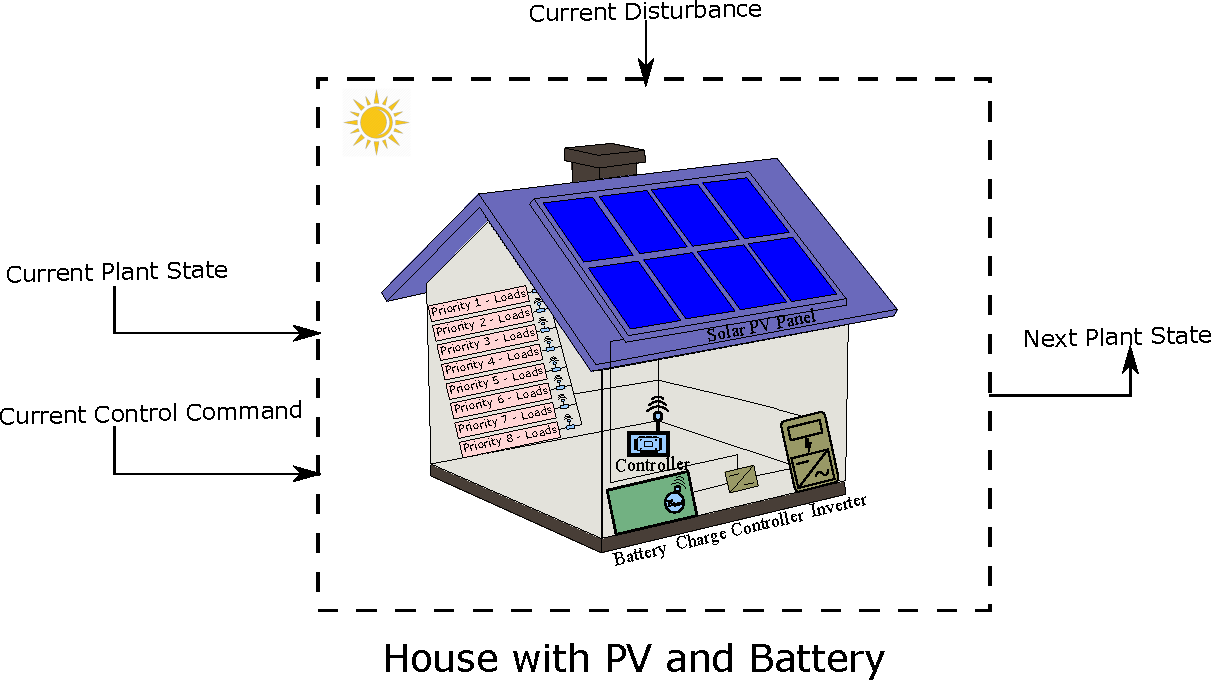
\includegraphics[scale=0.8]{SingleHouse_PV_Bat_Schematic.pdf}
	\caption{Schematic of Single house with PV, battery storage and prioritized loads.}
	\label{fig:SingleHouse_Schematic}
\end{figure}

Figure~\ref{fig:SingleHouse_Schematic} shows the schematic of a single house with PV, battery energy storage and prioritized loads. The prioritized load demands are the disturbances to the plant model and are taken from the Pecan Street Project. The prioritized loads are grouped as follows;

\begin{enumerate}
	\item Priority 1 Loads: Refrigerator, Freezer and Kitchen loads.
	\item Priority 2 Loads: Bedroom loads.
	\item Priority 3 Loads: Living room loads and office room loads.
	\item Priority 4 Loads: Clothes washer/dryer, garbage disposal and pumps.
	\item Priority 5 Loads: Security loads, Bathroom loads, dinning room loads and dish washer.
	\item Priority 6 Loads: Remaining rooms loads and outside lights.
	\item Priority 7 Loads: Aquarium load, lawn sprinklers and wine cooler
	\item Priority 8 Loads: Pool heating, water heater and jacuzzi.
\end{enumerate}

The above priority order is a choice and can be changed as per requirement of the community occupants.

\begin{figure}[htpb]
	\centering
	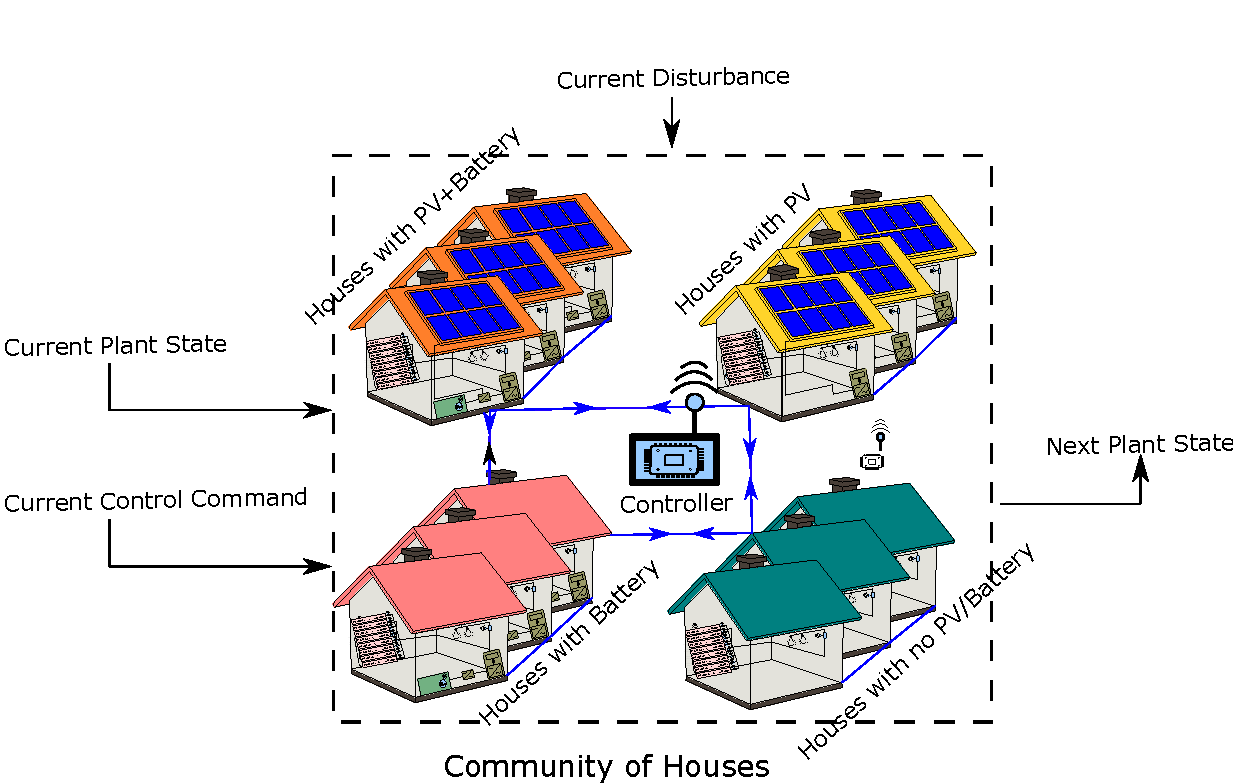
\includegraphics[scale=0.8]{CommunityHouses_Schematic.pdf}
	\caption{Schematic of community of heterogeneous house.}
	\label{fig:Community_Schematic}
\end{figure}

Figure~\ref{fig:Community_Schematic} shows the schematic of the community of heterogeneous houses i.e. the actual plant model and has the following attributes:

\begin{enumerate}
	\item Can simulate arbitrary $n$ number of houses
	\item The arbitrary $n$ number of houses can have an arbitrary number of houses with any combination of PV/Battery/none as local sources of energy within themselves.
	\item Thermal model of each house is simulated.
	\item The higher start-up current (which translates to high start-up power) of residential HVAC system is considered.
	\item Weather disturbances in the form of solar irradiance, ambient temperature and wind speed from NSRDB data sets alter the PV energy production potential of the PV modules if any in the community.
	\item Load disturbances in the form prioritized load demand from Pecan Street Project data sets act as load disturbances to the plant.
\end{enumerate}

The rest of the report is organized as follows: the system description and mathematical models of the system components are described in Section~\ref{section:PlantModel}. The formulation of the baseline and intelligent rule-based controllers are provided in the  Section~\ref{section:BaselineController} and Section~\ref{section:RuleBasedController} respectively. The results of the simulation study are presented and discussed in Section~\ref{section:PlantMATLABResults}. Finally, the main conclusions and future work are provided in Section~\ref{section:ConclusionFutureWork}.
\newpage

\section{Smart Community Plant Model}\label{section:PlantModel}

\subsection{Simulation Time}\label{subsection:SimulationTime}
Let $T=\{1,\dots,N_{t}\}$ be discrete time steps of simulation where $\Delta T = 10$mins between any two time indices $k+1$ and $k$, where $k \in T$.


\subsection{Houses}\label{subsection:Houses}
We have set of set $H = \{ \{H_{1}\},\{H_{2}\},\{H_{3}\},\{H_{4}\}\}$ of different types of houses. Where,

\begin{enumerate}
	\item Set of houses having PV+Battery ($H_{1}$) , $|H_{1}|=N_{1}$, where $N_{1}$ is the number of houses with PV+Battery.
	\item Set of houses having Battery ($H_{2}$) , $|H_{2}|=N_{2}$, where $N_{2}$ is the number of houses with Battery.
	\item Set of houses having PV ($H_{3}$) , $|H_{3}|=N_{3}$, where $N_{3}$ is the number of houses with PV.
	\item Set of houses having niether PV/Battery ($H_{4}$) , $|H_{4}|=N_{4}$, where $N_{4}$ is the number of houses without PV/Battery.	
\end{enumerate}

Also, let $H_{I}=\{1,2,\dots,N_{1}+N_{2}+N_{3}+N_{4}\}$ such that,

\begin{enumerate}
	\item If $i=\{1,\dots,N_{1}\} \in H_{I}$ then $h_{i} \in H_{1}$. 
	\item If $i=\{N_{1}+1,\dots,N_{1}+N_{2}\} \in H_{I}$ then $h_{i} \in H_{2}$. 
	\item If $i=\{N_{1}+N_{2}+1,\dots,N_{1}+N_{2}+N_{3}\} \in H_{I}$ then $h_{i} \in H_{3}$. 
	\item If $i=\{N_{1}+N_{2}+N_{3}+1,\dots,N_{1}+N_{2}+N_{3}+N_{4}\} \in H_{I}$ then $h_{i} \in H_{4}$. 	
\end{enumerate}

\subsection{House Thermal Model}\label{subsection:HouseThermalModel}

House thermal model model used in the plant is a $4^{\text{th}}$ order ODE model from \cite{CuiHybrid:2019} whose zero-order hold discretized version is used. But for simplicity we represent it as a $i^{\text{st}}$ order model as follows; for a house $h_{i}$, $i \in H_{I}$, i.e. $h_{i} \in H$, house temperature ($T_{i}^{h}$) is given as,
\begin{align}
	&T_{i}^{h}(k+1) = A T_{i}^{h}(k)+B u_{i}^{ac}(k)+D T_{am}(k)
\end{align}
where, A,B,D are the discrete time system constants. $u_{i}^{ac}$ is the AC on-off control command and $u_{i}^{ac} \in \{0,1\}$. Also, $Q_{ac}=\text{COP}.\text{P}^{ac,R}$, where COP is the coefficient of performance of the AC and $\text{P}^{ac,R}$ is the rated power of the AC, and $T_{am}$is the ambient temperature.

\subsection{Battery Energy Storage Model}\label{subsection:BatteryEnergyStorageModel}
Battery dynamics are modeled as a bucket of energy. For a house $h_{i} \in \{H_{1}, H_{2}\}$, the battery dynamics are given as ,
\begin{align}
	&E_{i}^{b}(k+1) = E_{i}^{b}(k)+\left[ \eta_{b}^{c} E_{i}^{b,c}(k)\right] +\left[  E_{i}^{b,dc}(k)\right] / \eta_{b}^{dc}
\end{align}
where, $E_{i}^{b}$ is the battery energy level, $E_{i}^{b,c}$ is the battery charging energy, $E_{i}^{b,dc}$ is the battery discharging energy, and $\eta_{b}^{c}$-$\eta_{b}^{dc}$ are the battery charging and discharging efficiencies respectively. Also, $E_{i}^{b} \in \{\underbar E^{b}, \bar E^{b} \}$, where $\underbar E^{b}$ is the maximum battery energy and $\bar E^{b}$ is the minimum battery energy. Also, we have,
\begin{align}
	E_{i}^{b,c}(k) &= c_{i}(k) \times min\{E_{i}^{av,c}(k), \left[ \bar E^{b}- E_{i}^{b}(k)\right]/\eta_{b}^{c}, \bar E^{b,c} \} \\
	E_{i}^{b,dc}(k) &= d_{i}(k) \times min\{E_{i}^{av,dc}(k), \left[ \bar  E_{i}^{b}(k)-E^{b}\right].\eta_{b}^{dc}, \bar E^{b,dc} \} \\	
\end{align}
where, $c_{i}$/$d_{i}$ are the battery charging/discharging control commands, $E_{i}^{av,c}$/$E_{i}^{av,dc}$ are the battery charging/discharging energy available, and $\bar E^{b,c}$/$\bar E^{b,cc}$ are the maximum battery charging/discharging energy during any time interval. Hence, we have $E_{i}^{b,c} \in \{0, \bar E^{b,c}\}$ and $E_{i}^{b,dc} \in \{0, \bar E^{b,dc}\}$. $E_{i}^{av,c}$ and $E_{i}^{av,dc}$ are computed during simulation and we will see them in detail in a subsequent section.

\subsection{House Loads}\label{subsection:HouseLoads}
Energy ($E_{d}$) used by any device ($d$) is the integral of its reated power ($P_{d}$) over the time step i.e. $E_{d}=P_{d} \times \Delta T$

\subsubsection{AC Load}\label{subsubsection:ACLoad}
All houses have air conditioners (AC) with rated power requirement of $P^{ac,R}$. Hence, the energy used by an AC for $i^{\text{th}}$ house between any two time steps is $E_{i}^{ac}=\{0,(P^{ac,R} \Delta T)/\eta_{inv}\}$. Where $\eta_{inv}$ is the inverter efficiency.

\subsubsection{Other Loads}\label{subsubsection:OtherLoads}
Other typical house load trajectories are taken as disturbance from Pecan Street Project data set. For a single house at time index $k$, the other load energy desired is $\bar E_{i}^{l} \in \mathbb{R}^{8}$, where the order of the device loads is in the descending order of priority as discussed earlier. Each priority load or group of loads is assumed to have its own circuit which can be independently switched on and off as needed. Hence the total load energy for house $i$ at time index $k$is given as, $E_{i}^{l}=(\left[  \bar E_{i}^{l}(k) \right] ^{T}.I)/\eta_{inv}$, where $I=[u_{i}^{l,1}\dots,u_{i}^{l,8}]^{T} \in \mathbb{R}^{8}$, where $u_{i}^{l,j}$, $j \in \{1,\dots,8\}$ is the on-off control command of the $j^{\text{th}}$ priority load.


\subsection{PV Energy Potential Model}\label{subsection:PVEnergyPotentialModel}
For a house $h_{i} \in \{H_{1}, H{3}\}$, the PV energy generation potential ($E_{i}^{pv}$) is given as, 

$E_{i}^{pv}(k)=f(\bar P_{i}^{pv,R},GHI(k),T_{am}(k), W_{s}(k))$. Where $P_{i}^{pv,R}$ is the rated power of the PV modules , $GHI$ is the solar irradiance, and $W_{s}$ is the wind speed. The function ($f()$) is a modified form from \cite{MastersRenewable:2013} with the inclusion of Faiman PV module temperature model \cite{FaimanAssessing:2008}, so that the effect of both $GHI$ and $T_{am}$, $W_{s}$ is observed on the PV generation potential.


\subsection{Overall Energy Simulation}\label{subsection:OverallEnergySimulation}
At any time index $k$, we have the total PV generation potential ($E_{H}^{pv}$) related to total PV energy used ($E_{H}^{pv,u}$) and total PV energy unused ($E_{H}^{pv,un}$) as follows,
\begin{align}
	E_{H}^{pv}(k) &= E_{H}^{pv,u}(k)+E_{H}^{pv,un}(k) \\
	E_{H}^{pv}(k) &= \sum_{i \in H_{I}} E_{i}^{pv}(k) \\	
	E_{H}^{pv,u}(k) &= \sum_{i \in H_{I}} E_{i}^{pv,u}(k) \\
	E_{H}^{pv,un}(k) &= \sum_{i \in H_{I}} E_{i}^{pv,un}(k) 
\end{align}
Now, the total load desired ($E_{H}^{L,d}$) is related to the total AC load desired ($E_{H}^{ac,d}$) and total other load desired ($E_{H}^{l,d}$) as follows,
\begin{align}
	E_{H}^{L,d}(k) &= E_{H}^{ac,d}(k)+E_{H}^{l,d}(k) \\
	E_{H}^{L,d}(k) &= \sum_{i \in H_{I}} E_{i}^{L,d}(k) \\	
	E_{H}^{ac,d}(k) &= \sum_{i \in H_{I}} E_{i}^{ac,d}(k) \\
	E_{H}^{l,d}(k) &= \sum_{i \in H_{I}} E_{i}^{l,d}(k) 
\end{align}
where, $E_{i}^{l,d} =E_{i}^{l}$.
Also, the total battery charging energy ($E_{H}^{b,c}$) and total battery discharging energy ($E_{H}^{b,dc}$) are given as,
\begin{align}	
	E_{H}^{b,c}(k) &= \sum_{i \in \{H_{1},H_{2}\}} E_{i}^{b,c}(k) \\
	E_{H}^{b,dc}(k) &= \sum_{i \in \{H_{1},H_{2}\}} E_{i}^{b,dc}(k) 
\end{align}
Now, we also have the following for energy balance of the community,
\begin{align}	
	E_{H}^{pv,u}(k) &= E_{H}^{L,a}(k)+E_{H}^{b,c}(k)-E_{H}^{b,dc}(k)\\
	E_{H}^{L,a}(k) &= \sum_{i \in H_{I}} E_{i}^{l,a}(k) 
\end{align}
where, $E_{H}^{L,a}$ is the total load energy supplied to the all the houses, and $E_{i}^{L,a}$ is the total load energy supplied to the $i^{\text{th}}$ house. The supply of $E_{i}^{l,a}$ depends on the energy and power constraint violation as follows,
\begin{align}
	E_{i}^{l,a}(k)= & 
	\begin{cases}
		0 \; , & \text{if, Energy AND Power contraints are violated}  \\
		E_{i}^{l,d} \; , & \text{otherwise} \\
	\end{cases}
\end{align}
Now, to determine the violation of energy, we compute total available energy ($E_{H}^{av}$) and total energy desired ($E_{H}^{d}$) as follows,
\begin{align}	
	E_{H}^{av}(k) &= E_{H}^{pv,av}(k)+E_{h}^{b,dc,p}(k)\\
	E_{H}^{b,dc,p}(k) &= \sum_{i \in \{H_{1},H_{2}\}} E_{i}^{b,dc,p}(k)\\
	E_{i}^{b,dc,p}(k) &= d_{i}(k) \times min\left\lbrace \left[ \bar  E_{i}^{b}(k)-E^{b}\right].\eta_{b}^{dc}, \bar E^{b,dc} \right\rbrace  \\
	E_{H}^{d}(k) &= E_{H}^{L,d}+E_{H}^{b,c,p}\\
	E_{H}^{b,c,p}(k) &= \sum_{i \in \{H_{1},H_{2}\}} E_{i}^{b,c,p}(k)\\
	E_{i}^{b,c,p}(k) &= c_{i}(k) \times min\left\lbrace \left[E^{b}- \bar  E_{i}^{b}(k)\right]/\eta_{b}^{dc}, \bar E^{b,c} \right\rbrace 
\end{align}
where, $E_{H}^{b,c,p}$/$E_{H}^{b,dc,p}$ are the battery possible charging and discharging energies for all the houses and the $i^{\text{th}}$ house respectively, and $E_{i}^{b,c,p}$/$E_{i}^{b,dc,p}$ are the battery possible discharging and discharging energies for all the houses and the $i^{\text{th}}$ house respectively. We can now compute energy constraint violation as follows,

\begin{align}
	\text{Energy Constraint Violation }(k)= & 
	\begin{cases}
		\text{Yes} \; , & \text{if } E_{mis}(k)<0  \\
		\text{No} \; , & \text{otherwise} \\
	\end{cases}\\
	E_{mis}(k)=E_{H}^{av}-E_{H}^{d}
\end{align}

Now, to determine the violation of the power constraint, we compute the  total power available and toal start-up power required by turning on ACs as follows,
\begin{align}	
	P_{H}^{av}(k) &= E_{H}^{pv,av}/ \Delta T + \left\lbrace \sum_{i \in \{H_{1},H_{2}\}} d_{i}(k) \right\rbrace  . \bar P^{b,dc}\\
	P_{H}^{ac,su,req}(k) &= \left\lbrace \sum_{i \in H_{I}}\left[ u_{i}^{ac}(k) - u_{i}^{ac}(k-1) \right]  \right\rbrace . \bar P^{ac,su} 
\end{align}
where, $\bar P^{b,dc}$ is the maximum discharge power of battery for short duration, and $\bar P^{ac,su} $ is the start-up power of an AC. We can now compute power constraint violation as follows,
\begin{align}
	\text{Power Constraint Violation }(k)= & 
	\begin{cases}
		\text{Yes} \; , & \text{if } P_{mis}(k)<0  \\
		\text{No} \; , & \text{otherwise} \\
	\end{cases}\\
	P_{mis}(k)=P_{H}^{av}-P_{H}^{ac,su,req}
\end{align}
If there is negative energy or power mismatch, then the circuit voltages would collapse leading to no energy transfer for utilization, similarly if there is none/positive energy or power mismatch then energy transfer happens and the desired loads are served.

\newpage

\section{Smart Community Baseline Controller}\label{section:BaselineController}
The action of this controller can be decomposed into three independent local controllers: AC thermostat controller, battery controller and other loads controller.

The AC thermostat controller produces the AC on-off command ($u_{i}^{ac}$) as follows,
\begin{align}
	u_{i}^{ac}(k)= & 
	\begin{cases}
		1 \; , & \text{if } T_{i}^{h}\geq \bar T^{h} \\
		0 \; , & \text{if } T_{i}^{h}\leq \underbar T^{h} \\
		u_{i}^{ac}(k-1) \; , & \text{otherwise } 
	\end{cases}
\end{align}
where, $\bar T^{h}$ is the upper level of the thermostat temperature band, and $\underbar T^{h}$ is the lower level of the thermostat temperature band.

The battery logic controller produces battery charging ($c_{i}$) and discharging commands ($d_{i}$) as follows,
\begin{align}
	c(i)(k)= & 
	\begin{cases}
		1 \; , & \text{if } E_{H}^{pv}-E_{h}^{L,d}\geq0 \\
		0 \; , & \text{otherwise} \\
	\end{cases}\\
	d(i)(k)= & 
	\begin{cases}
		1 \; , & \text{if } E_{H}^{pv}-E_{h}^{L,d}<0 \\
		0 \; , & \text{otherwise} \\
	\end{cases}
\end{align}

The other loads controller produces the on-off command ($u_{i}^{l,j}$) for the prioritized loads as follows,
\begin{align}
	u_{i}^{l,j}(k)= & 
	\begin{cases}
		1 \; , & \text{if }  \left[ \bar E_{i}^{l}(j)\right] (k) \\
		0 \; , & \text{otherwise} \\
	\end{cases}
\end{align}
\newpage

\section{Smart Community Intelligent Rule-Based Controller}\label{section:RuleBasedController}
The role of the intelligent rule-based controller is to find a way if possible to avoid the violations of the energy and power constraints. It avoids energy constraint violation by shedding $|E_{mis}|$ through devices (turned on ACs, charging batteries and other loads) whenever possible, and avoids power constraint violation by shedding $|P_{mis}|$ through turning on ACs. The order of priority for shedding $|E_{mis}|$ is : Priority [Battery Charging] < Priority [Turning on ACs] < Priority [Turned on ACs] < Priority [Other loads]. While the only way to avoid power constraint violation is by controlling the the turning on ACs. The logic of this controller is straight forward and is accessible by just going through the code. Moreover, the shedding of charging batteries and turned on ACs and turning on ACs is random if lesser than the current devices in their particular states are required to meet the energy and power constraints.


\newpage

\section{Smart Community Plant - MATLAB and Python Code Description}\label{section:PlantMATLABPython}

The description of the scripts and functions and classes for the smart community plant simulation in MATLAB and Python is available in the Excel spreadsheets along with the code repository is linked below:

\begin{itemize}
	\item \href{{run:./ExcelFiles/MATLABFunctions.xlsx}}{MATLAB code description.}
	\item \href{{run:./ExcelFiles/PythonModules.xlsx}}{Python code description.}
	\item \url{https://github.com/ninadkgaikwad/SmartCommunityPlantModel} 
\end{itemize}


Note: For successful opening of links from within this document open document in ADOBE Reader.



\newpage

\section{Smart Community Plant - MATLAB Results}\label{section:PlantMATLABResults}
The period selected for simulation is the time hurricane Irma passed over Gainesville, FL, USA, starting from its landfall on Sept. 11, 2017, to Sept. 17, 2017. Weather data is obtained from National Solar Radiation Database (\url{nsrdb.nrel.gov}) and the load data is obtained from Pecan Street Project (\url{https://www.pecanstreet.org
}). The simulations are run for 7 days starting at 00:00~hours (midnight) at day 1 (September 11, 2017)  with a time step of 10 minutes ($\Delta T_{s}=10 $) with all battery initial states at $\bar E_{bat}$ (i.e., $E_{bat}^{i}(0)=\bar E_{bat}$) and  internal house temperatures are randomly initialized between maximum and minimum set-point temperatures of the AC thermostat, $\underbar T_{h}\leq T_{h}^{i}(k)\leq \bar T_{h}$, the house thermal dynamics are based on the linear model given by~\cite{CuiHybrid:2019}, which models a typical, detached, two-story house in the USA.

\newpage

\begin{figure*}[!t]
	\centering
	\begin{subfigure}[t]{0.48\textwidth}
		\centering
		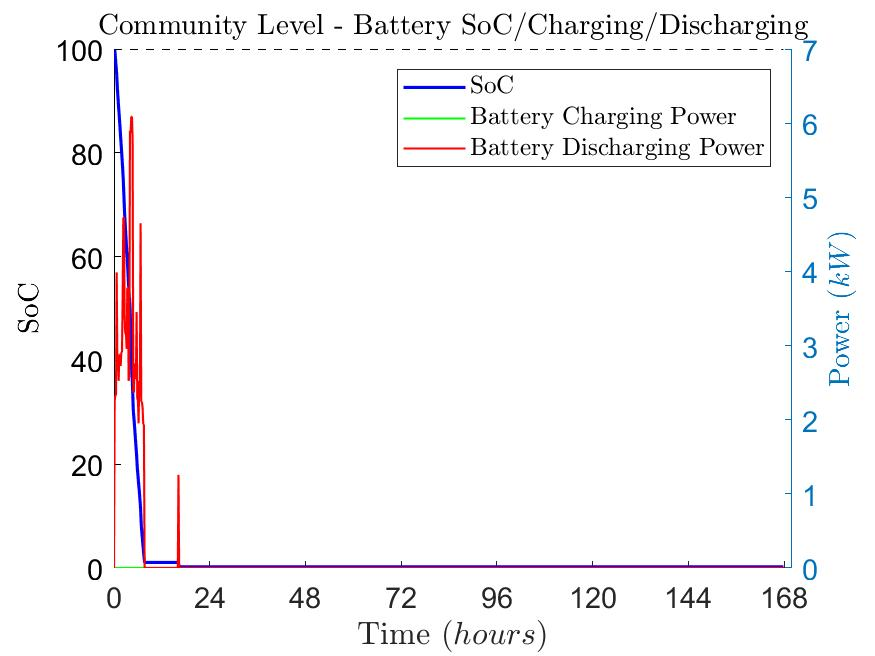
\includegraphics[scale=0.3]{Gainesville_BaseLine_7DayTest_SC_PVBat1_Bat1_PV1_None1_SCL2_Community_Bat_SoC_C_DisC.JPG}
		\caption{Battery SoC.}
		\label{fig:Bat_1}
	\end{subfigure}
	\begin{subfigure}[t]{0.48\textwidth}
		\centering
		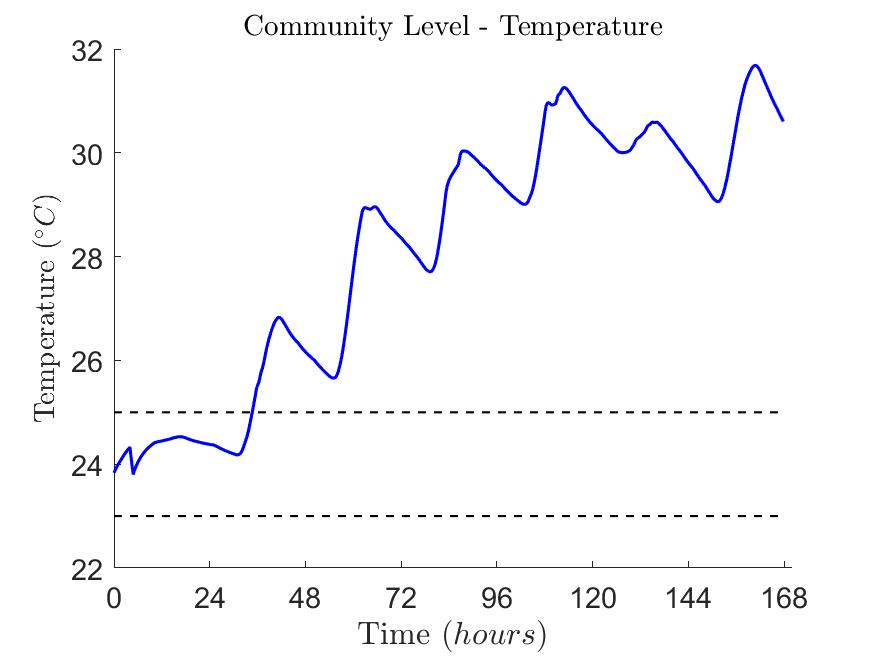
\includegraphics[scale=0.3]{Gainesville_BaseLine_7DayTest_SC_PVBat1_Bat1_PV1_None1_SCL2_Community_Temperature.JPG}
		\caption{House Temperature.}
		\label{fig:Temp_1}
	\end{subfigure}
	
	\begin{subfigure}[t]{0.48\textwidth}
		\centering
		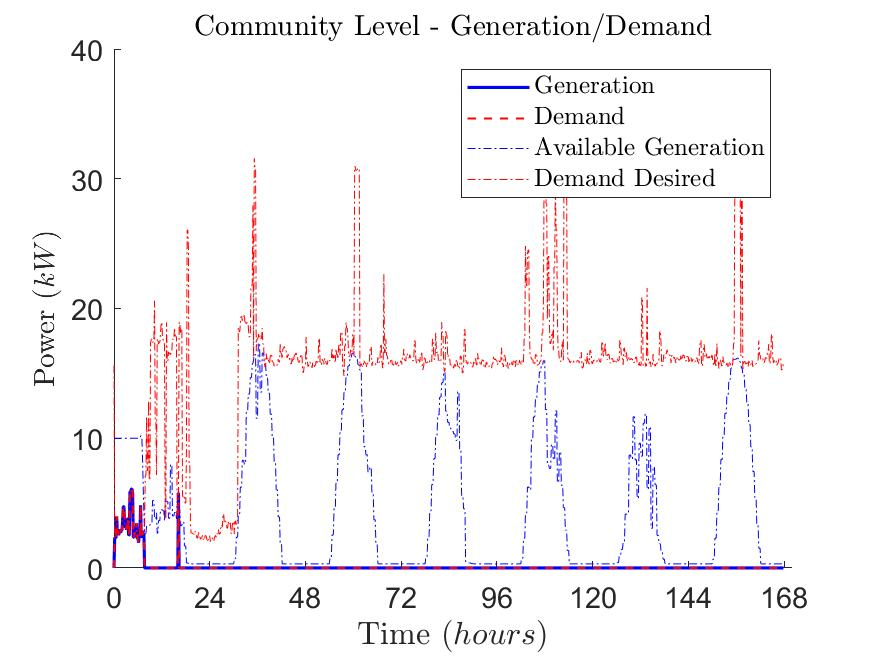
\includegraphics[scale=0.3]{Gainesville_BaseLine_7DayTest_SC_PVBat1_Bat1_PV1_None1_SCL2_Community_P_Generated_Demand.JPG}
		\caption{Generation and Load Demand.}
		\label{fig:GenDemand_1}
	\end{subfigure} 
	\begin{subfigure}[t]{0.48\textwidth}
		\centering
		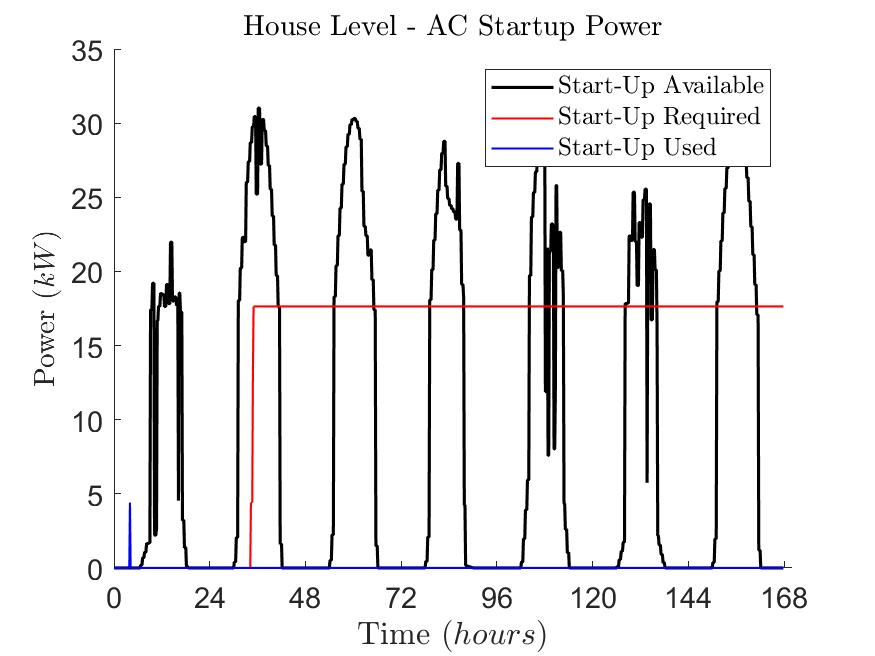
\includegraphics[scale=0.3]{Gainesville_BaseLine_7DayTest_SC_PVBat1_Bat1_PV1_None1_SCL2_Community_AC_StartUpPower_Av_Req_U.JPG}
		\caption{AC Start-up Power.}
		\label{fig:AcStartUp_1}
	\end{subfigure} 
	\caption{Baseline controller plots.}
	\label{fig:Results_Baseline}
\end{figure*}

Figure~\ref{fig:Results_Baseline} shows the simulation result when baseline controller is used. As we can see from Figure~\ref{fig:Bat_1} the house batteries in the community deplete their store energy with the first 24 hours of the outage and are never able to recharge fully owing to the lack of control on secondary loads and inability to start-up only those many AC's for which start-up power is available, see Figure~\ref{fig:GenDemand_1} and Figure~\ref{fig:AcStartUp_1}. We can see the run-away house temperatures of the community due to no energy transfer in the entire circuit as result of power and energy constraint violations in Figure~\ref{fig:Temp_1}. Hence, we can say that a community of houses, with its current baseline controllers cannot provide resiliency during an extended outage in spite of having the required generation resources.

\newpage

\begin{figure*}[!t]
	\centering
	\begin{subfigure}[t]{0.48\textwidth}
		\centering
		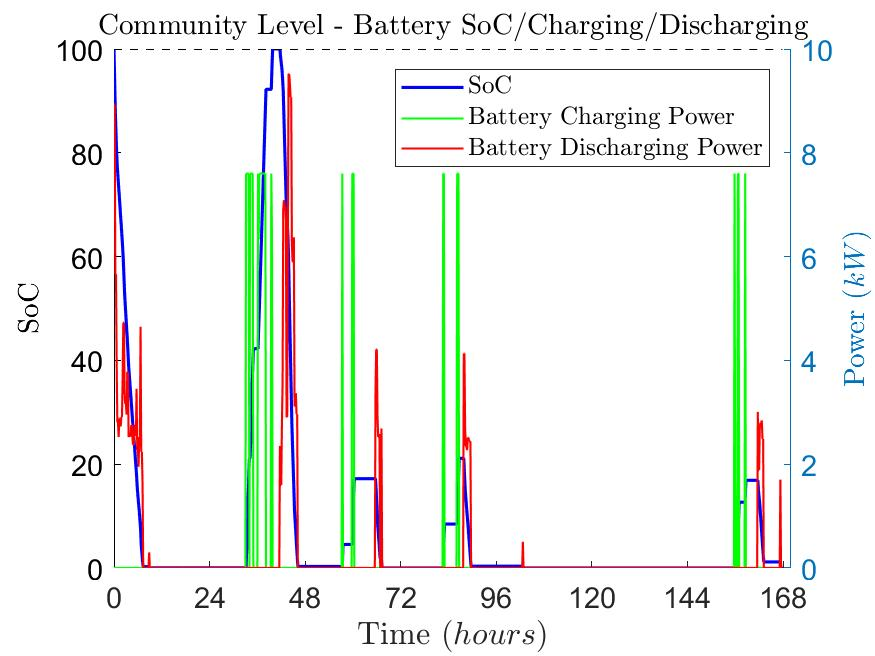
\includegraphics[scale=0.3]{Gainesville_BaseLine_7DayTest_SC_PVBat1_Bat1_PV1_None1_SCL1_Community_Bat_SoC_C_DisC.JPG}
		\caption{Battery SoC.}
		\label{fig:Bat_2}
	\end{subfigure}
	\begin{subfigure}[t]{0.48\textwidth}
		\centering
		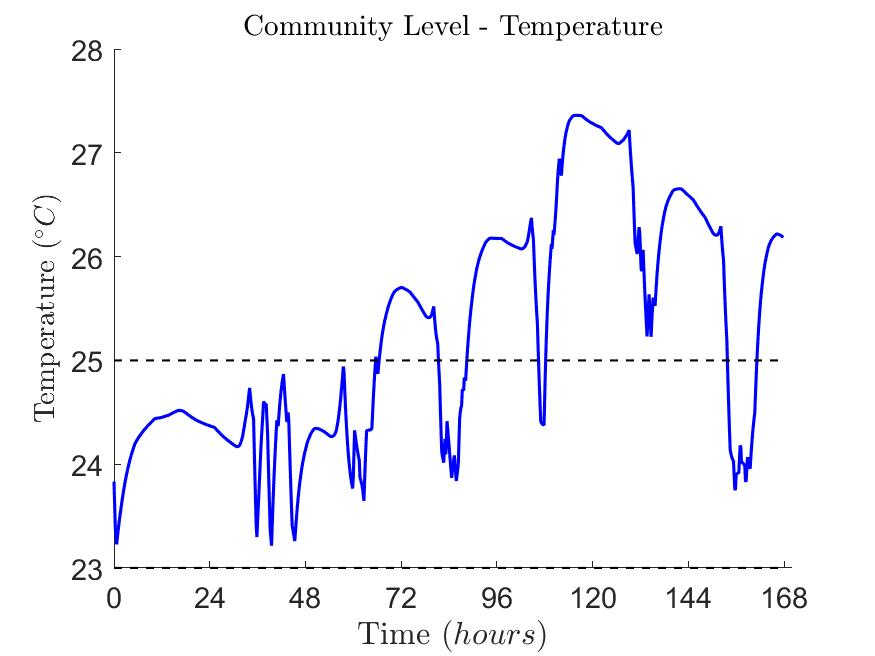
\includegraphics[scale=0.3]{Gainesville_BaseLine_7DayTest_SC_PVBat1_Bat1_PV1_None1_SCL1_Community_Temperature.JPG}
		\caption{House Temperature.}
		\label{fig:Temp_2}
	\end{subfigure}
	
	\begin{subfigure}[t]{0.48\textwidth}
		\centering
		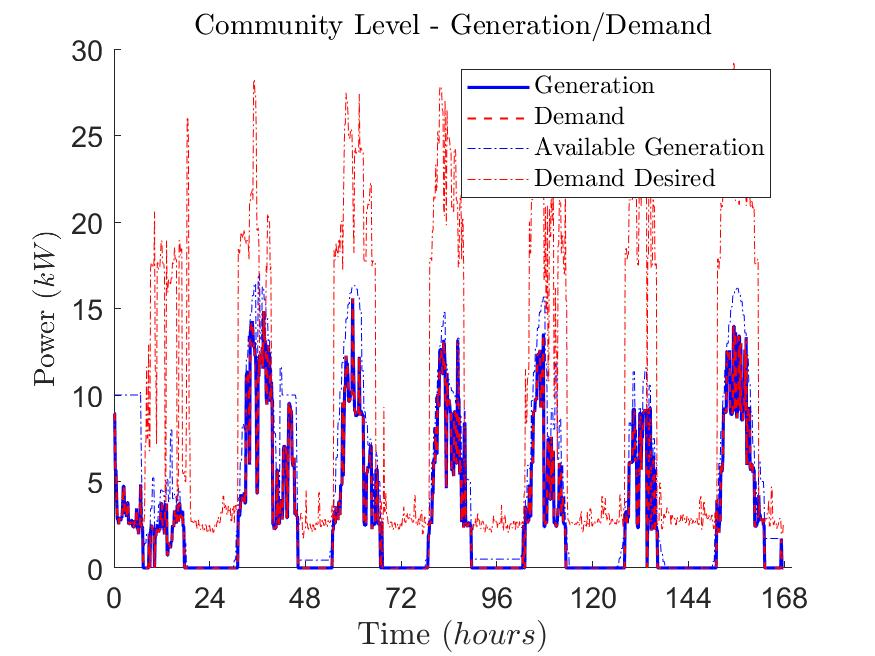
\includegraphics[scale=0.3]{Gainesville_BaseLine_7DayTest_SC_PVBat1_Bat1_PV1_None1_SCL1_Community_P_Generated_Demand.JPG}
		\caption{Generation and Load Demand.}
		\label{fig:GenDemand_2}
	\end{subfigure} 
	\begin{subfigure}[t]{0.48\textwidth}
		\centering
		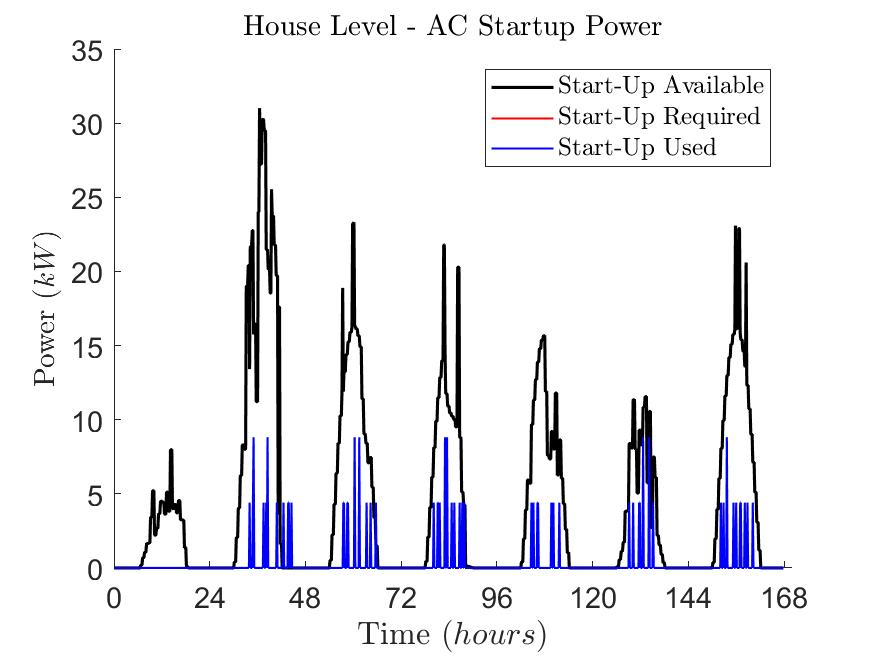
\includegraphics[scale=0.3]{Gainesville_BaseLine_7DayTest_SC_PVBat1_Bat1_PV1_None1_SCL1_Community_AC_StartUpPower_Av_Req_U.JPG}
		\caption{AC Start-up Power.}
		\label{fig:AcStartUp_2}
	\end{subfigure} 
	\caption{Intelligent Rule-Based controller plots.}
	\label{fig:RuleBased}
\end{figure*}

Figure~\ref{fig:RuleBased} shows the simulation result when Intelligent Rule-Based controller is used. As we can see from Figure~\ref{fig:Bat_2} the house batteries in the community do better than the baseline controller scenario and are able to recharge to some degree over the period of simulation. This is made possible through prioritized control of secondary loads and the ability to start-up only those many AC's for which start-up power is available, see Figure~\ref{fig:GenDemand_2} and Figure~\ref{fig:AcStartUp_2}. We can see the house temperatures of the community being maintained up until 72 hours into the outage and only run-away when the battery is not recharged  later in the simulation period, see Figure~\ref{fig:Temp_2}. The power and energy constraint violations caused by the Intelligent Rule-Based controller are significantly less than that caused by the baseline controller. Hence, we can say that a community of houses, with the Intelligent Rule-Based controller can provide some degree of resiliency during an extended outage. However, a more intelligent controller based in Model Predictive Control (MPC) or Reinforcement Learning (RL) can perform better owing to the ability to utilize future disturbance information and being based on the construct of optimization.

\newpage

\section{Conclusion and Future Work}\label{section:ConclusionFutureWork}
A controllable plant model of a community of houses has been developed which simulates the energy production and consumption of a heterogeneous mixture of houses which can have solar PV and/or battery energy storage or none as sources of energy, along with simulating the thermal dynamics of the houses it also incorporates the higher start-up power required by residential HVAC systems, in an off-grid mode during extended outages. The weather and household load demands form the disturbance to the plant model. Functionality for preprocessing and ingesting weather data from NSRDB and household load demand from Pecan Street Project have also been developed. Two controllers: baseline and intelligent rule-based have been developed and the results of closed-loop simulations using these controllers on the plant illustrate the proper working of the plant. All the pieces of code necessary for the closed-loop simulations are complete in MATLAB, while in Python some more functionality has to still be coded up.

For future work, we would like to complete the remaining pieces of code in Python. Furthermore, we would like to add Electric Vehicles (EV) as a second source of battery energy storage with its disturbance of being present and connected in the house in both MATLAB and Python.

\newpage

\section{Acknowledgement}\label{section:Acknowledgement}
A special thanks to Christopher Crouch the UG research scholar of DiCE Lab who has worked on developing the Python code for the plant model based of my MATLAB code.

\bibliographystyle{IEEEtran}
\bibliography{./BibFolder/BiBFile}
	
\end{document}















